\index{general}{Domain Decomposition}

Let us assume that we want ro run a simulation of the whole Earth mantle
with a constant resolution of $5\text{km}$. The volume of the mantle is
\[
V_{mantle}=\frac{4}{3}\pi (R_{out}^3-R_{in}^3) \simeq  10^{12}  km^3
\]
while the volume of an element is $V_{e} = 125 \text{km}^3$ (this is 
only an average since the tesselation of a hollow sphere with 
hexahedra yields elements which are not all similar \cite{thie18}).
Consequently, the number of cells needed to discretise the mantle
is 
\[
N_{el}=\frac{V_{mantle}}{V_{e}}\simeq 8\times 10^9
\]
We know that the matrix size is approx. 4 times the number of elements in 3D:
\[
N\simeq 25 \times 10^9
\]
Using between 9 and 125 particles per element (a very conservative number),
the total number of particles is then
\[
N_{particles}  \geq 10^{10}
\]
The unescapable conclusion is that high-resolution 3D 
calculations 
 have a very large memory footprint and require extremely long computational times.

The only way to overcome this problem is by resorting to 
using supercomputers with many processors and large memory capacities.

The idea behind parallel programming is to have each processor carry out 
only a subset of the total number of operations required. In order to reduce 
the memory footprint on each processor, only a subset of the computational
mesh is known by each: one speaks then of domain decomposition.

An example of such a large parallel calculation of 3D convection with 
domain decomposition in a spherical shell can be found in \cite{krhb12}:

\begin{center}
a)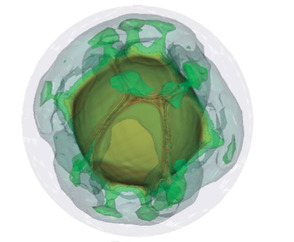
\includegraphics[width=7cm]{images/krhb2}
b)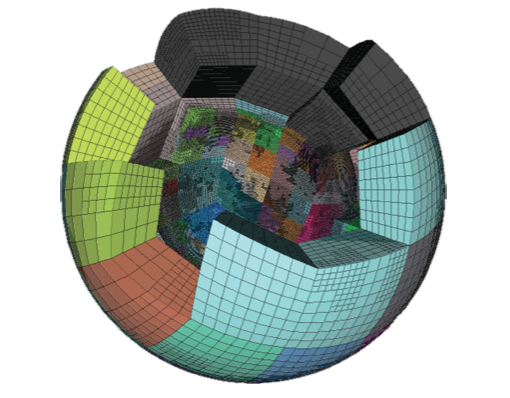
\includegraphics[width=7cm]{images/krhb1} \\
{\captionfont a)Isocontours of the temperature field; b) Partitioning of the domain onto 512 proc. The mesh counts 1,424,176 cells. The solution has approximately 54 million unknowns (39 million vel., 1.7 million press., and 13 million temp.)
}
\end{center}


\Literature:
\begin{itemize}
\item Three parallel iterative solvers for the Stokes system, discretized by low order 
tetrahedral elements, are compared with respect to their numerical efficiency and their 
scalability running on up to 786,432 parallel threads \cite{gmhj15}
\end{itemize}
